\question[4]
Gib für den abgebildeten Graphen die Implementierung in Python als Adjazenzmatrix an.
Die Knoten a,b,c,.. sind auf die Indizes 0,1,2,... abgebildet.

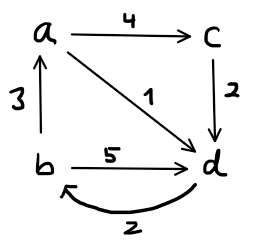
\includegraphics[height=4cm]{\pfad/Graphen/Aufgaben/adjazenzmatrix_05b/adjazenzmatrix_05b.png}
\begin{solutionbox}{5cm}
\begin{lstlisting}
inf = float('inf')
G = [[0,inf,4,1],
     [3,0,inf,5],
     [inf,inf,0,2],
     [inf,2,inf,0]]
\end{lstlisting}
\end{solutionbox}
